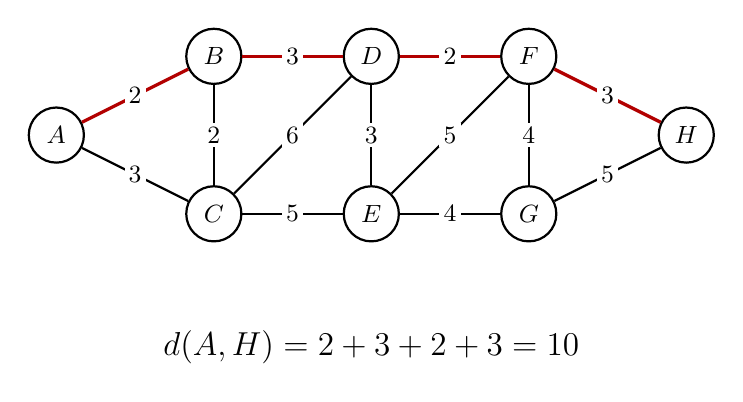
\begin{tikzpicture}[
    scale=1,
    every node/.style={font=\small},
    vertex/.style={draw, circle, thick, minimum size=7mm, inner sep=0pt},
    edge/.style={thick},
    selected/.style={draw=red!70!black, very thick},
    weight/.style={fill=white, inner sep=1.5pt}
]

% vrcholy
\node[vertex] (A) at (0,1.5) {$A$};
\node[vertex] (B) at (2,2.5) {$B$};
\node[vertex] (C) at (2,0.5) {$C$};
\node[vertex] (D) at (4,2.5) {$D$};
\node[vertex] (E) at (4,0.5) {$E$};
\node[vertex] (F) at (6,2.5) {$F$};
\node[vertex] (G) at (6,0.5) {$G$};
\node[vertex] (H) at (8,1.5) {$H$};

% běžné hrany
\draw[edge] (A) -- node[weight] {$3$} (C);
\draw[edge] (B) -- node[weight] {$2$} (C);
\draw[edge] (C) -- node[weight] {$5$} (E);
\draw[edge] (C) -- node[weight] {$6$} (D);
\draw[edge] (D) -- node[weight] {$3$} (E);
\draw[edge] (E) -- node[weight] {$4$} (G);
\draw[edge] (E) -- node[weight] {$5$} (F);
\draw[edge] (F) -- node[weight] {$4$} (G);
\draw[edge] (G) -- node[weight] {$5$} (H);

% vyznačená nejkratší cesta A-B-D-F-H
\draw[selected] (A) -- node[weight] {$2$} (B);
\draw[selected] (B) -- node[weight] {$3$} (D);
\draw[selected] (D) -- node[weight] {$2$} (F);
\draw[selected] (F) -- node[weight] {$3$} (H);

% popisek vzdálenosti
\node[align=center] at (4,-1.2) {\large $\displaystyle d(A,H)=2+3+2+3=10$};

\end{tikzpicture}